\documentclass[convert={density=300,outext=.png}]{standalone}
\usepackage{tikz}
\usetikzlibrary{shapes,arrows,decorations,decorations.pathmorphing,arrows.meta,patterns,decorations.markings}

\begin{document}
%% Use \usepackage{tikz}
%% Use \usetikzlibrary{shapes,arrows,decorations, decorations.pathmorphing,arrows.meta,patterns}
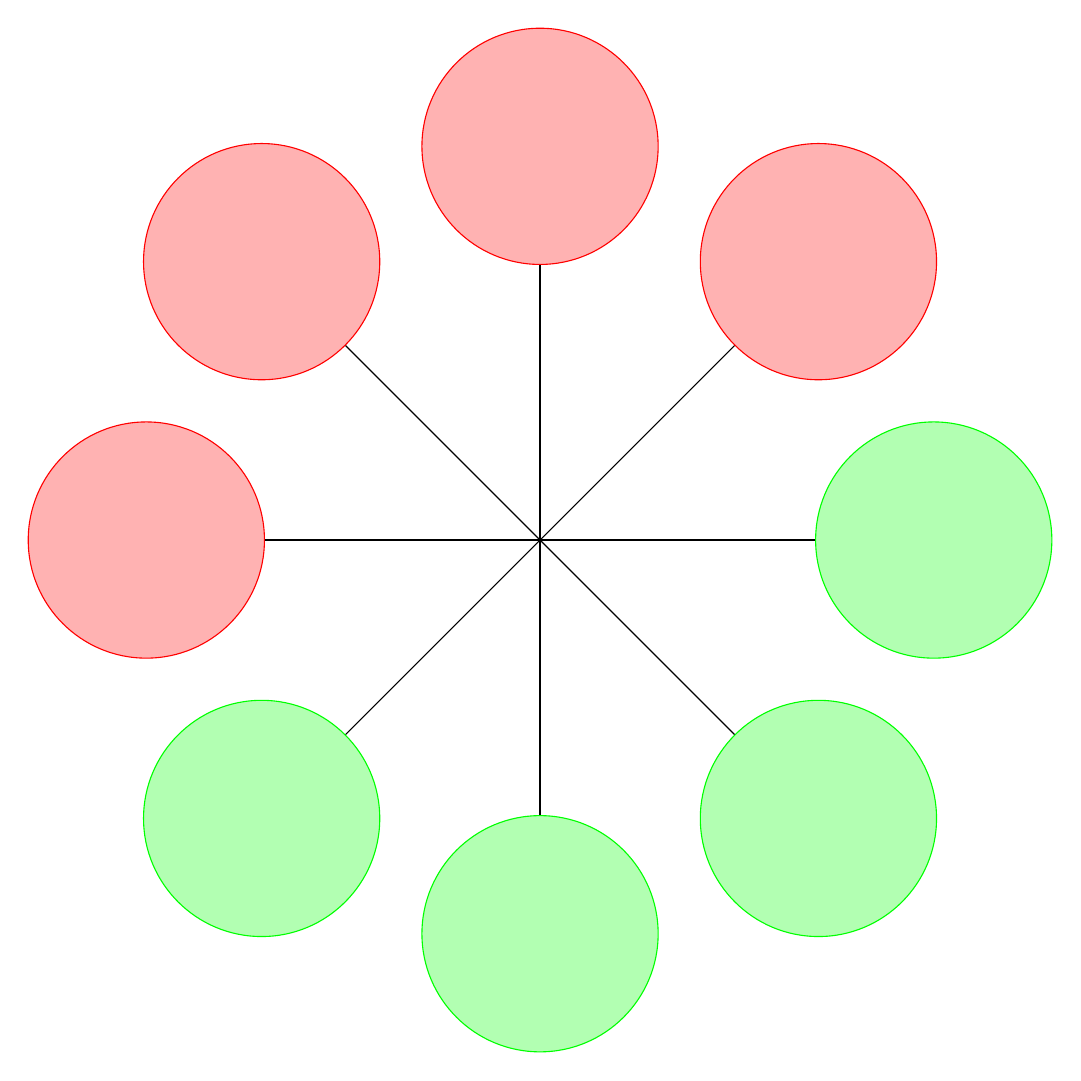
\begin{tikzpicture}[scale=1.0000]
	\tikzstyle{every node}=[scale=1.0000]
	
	%%Created with tikzpy
	
	\draw  (5.0000,0.0000,0.0000) -- (-5.0000,0.0000,0.0000);
	\draw  (3.5355,-3.5355,0.0000) -- (-3.5355,3.5355,0.0000);
	\draw  (0.0000,-5.0000,0.0000) -- (-0.0000,5.0000,0.0000);
	\draw  (-3.5355,-3.5355,0.0000) -- (3.5355,3.5355,0.0000);
	\draw [green , fill= green!30 ,]  (5.0000,0.0000,0.0000) circle [radius=1.5000];
	\draw [red , fill= red!30 ,]  (-5.0000,0.0000,0.0000) circle [radius=1.5000];
	\draw [green , fill= green!30 ,]  (3.5355,-3.5355,0.0000) circle [radius=1.5000];
	\draw [red , fill= red!30 ,]  (-3.5355,3.5355,0.0000) circle [radius=1.5000];
	\draw [green , fill= green!30 ,]  (0.0000,-5.0000,0.0000) circle [radius=1.5000];
	\draw [red , fill= red!30 ,]  (-0.0000,5.0000,0.0000) circle [radius=1.5000];
	\draw [green , fill= green!30 ,]  (-3.5355,-3.5355,0.0000) circle [radius=1.5000];
	\draw [red , fill= red!30 ,]  (3.5355,3.5355,0.0000) circle [radius=1.5000];

\end{tikzpicture}
\end{document}
